
\maketitle

\section{changelog}
\input{git.tex}


\section{Idea}

The fundamental idea behind this strategy is to assign each thread to a subset of the workspace. Each thread will manage it's own kd-tree containing all sampled points within it's assigned sub-space. 

\begin{figure}[H]
\begin{centering}
    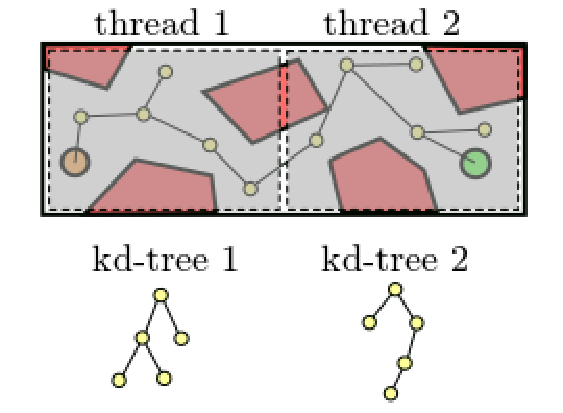
\includegraphics[scale=1]{fig/thread_kdtree}
    \caption{Division Strategy}
\end{centering}
\end{figure}

\section{Sampling}

Sampling should be rather straightforward. Mutsuo Saito and Makoto Matsumoto have realsed CUDA codes for using Merseinne Twister to generate uniform random samples on the GPU. Their webpage for this implementation (MTGP) is at \url{http://www.math.sci.hiroshima-u.ac.jp/~m-mat/MT/MTGP/index.html}

\subsection{Implementation}

The kernel uses a block of memory to maintain the state of the algorithm, and outputs an array of random numbers to another block of memory. 

\begin{figure}[H]
\begin{centering}
    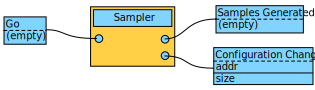
\includegraphics[scale=1]{fig/blocks/sampler}
    \caption{Sampler Block}
\end{centering}
\end{figure}

The sampler block has a single slot which listens for a signal with an empty message. When this slot is activated the MTGP kernel is run, and a signal is emitted. The emitted signal contains an empty message. The sampler block also emits a signal on configuration changes, which occur by calling class methods to change the size of the block of random numbers that are generated. This signal carries information about the start address and size of the block of random numbers. Downstream blocks should cache this information and use it to read samples when the sampler emits it's other signal.


\section{Nearest Neighbor}


\subsection{Single query}
For a single query composing of a single sample against a single data set, it's hard to get a linear speed-up in the number of threads. The reason is that $\log n$ efficiency is achieved by a search tree, which yields inherently serial queries. One way to parallelize a search tree is to store some amount of a subtree consecutively in memory. 

Traditionally, we store a binary search tree where a single node points to two child nodes. We can generalize this in two ways. 

\subsection{Reduction of $n$-ary search tree}
Instead of a binary search tree, we can store a $n$-ary search tree, where a single node points to some $n$- children. Stepping through that node will require searching through it's list of children to find out which child to step to. This amounts to a reduction, which can be sped up to $\log T$ for $T$ threads. 

\begin{figure}[H]
\begin{centering}
    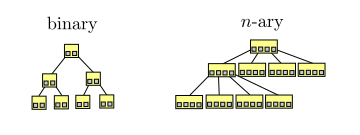
\includegraphics[scale=1]{fig/nary_search_tree}
    \caption{$n$-ary Search Tree}
    \label{fig:nary_tree}
\end{centering}
\end{figure}

\subsection{Storing subtree}
Additionally, we can store some depth of a node and it's children continuously in memory, essentially creating a macro-tree where each node is composed of some number of nodes of the underlying tree. We can can assign one thread to pre-expand all ancestors of a particular node to some depth, and then use a single thread to traverse that depth.

 \begin{figure}[H]
\begin{centering}
    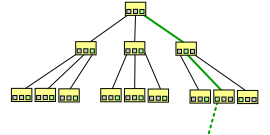
\includegraphics[scale=1]{fig/ddepth_macro_tree}
    \caption{$d$-depth Search Tree}
    \label{fig:ddepth_tree}
\end{centering}
\end{figure}

In figure \ref{fig:ddepth_tree} with a 3-ary tree and macro-node depth of 3, we use 7 threads to determine which child pointer to follow for each of the 7 micro-nodes in the macro node (marked with the light green). Then we use a single thread to step through the results (the green lines). This is ``wasteful'' in the sense that the result computed by 4 of the threads is left unused. 

\subsection{Multi-query}
We can potentially do nearest neighbor search in the same way as a single-thread RRT*, by searching over all nodes for the nearest neighbor. This can be somewhat of a challenge though if each thread has it's own kd tree, because we first need to find the nearest non-empty bin(s), and then find the nearest nodes in those bins. Therefore we may want to super-impose an additional data structure on top of the thread-divisioned kd trees.  

Assuming that the number of threads is unchanging then we can store a quad-tree to index the threads' kd-trees. This will use a constant amount of space and we can further speed up future searches if, at the end of each search, the thread stores the distance from it's bin to the bin where the nearest node was found. Subsequent searches can start from that depth in the kd-tree, up until the thread starts finding nearest nodes in the neighboring bins. Each nearest neighbor search will always have to at least look in it's own bin, and all of its neighboring bins, because nodes near the edge of the bin could be closer to nodes of the neighboring bin than nodes of it's own bin.

\begin{figure}[H]
\begin{centering}
    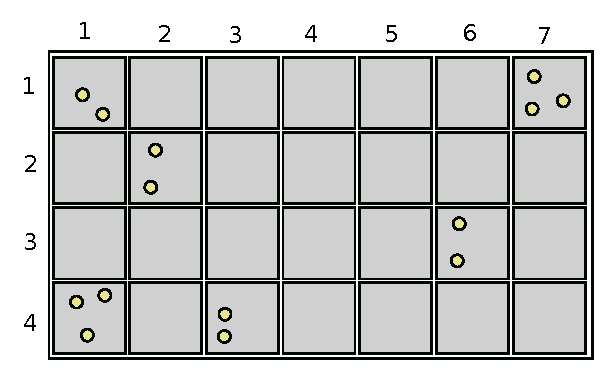
\includegraphics[scale=1]{fig/nonempty_search}
    \caption{Non-empty Search}
    \label{fig:nonempty}
\end{centering}
\end{figure}


We'd like a data structure which will allow us to efficiently find the nearest bin(s) which contain at least one node. We'd like this structure to provide efficient queries for all bins. While it is true that the number of threads will be constant (and thus, searching over all of them will be constant time), there may be thousands of threads and we can potentially see a significant improvement by an added index. 

Consider figure \ref{fig:nonempty}. If we generate a sample in bin (2,4), then we only need to search bins (2,2), (4,3), and (3,6) for the nearest node. If we generate a sample in bin (1,1), we only need to search bins (1,1) and (2,2). In the worst case, we would have to search all the bins on the perimeter of the workspace. 

\subsection{Full Bins}

When all bins contain at least one node, then the nearest node to a sample will be in the bin where the sample was generated, or any of the eight other bins around it. We can assign separate threads to search each of the trees, storing all the results in shared memory, and then running a reduction on it. 

\subsection{Prior to full bins}

\subsubsection{Index Idea}

Here is an idea. For each bin, store an integer corresponding to the unilateral distance (measured in number of bins on the longest edge) to the nearest non-empty bin. For bin (4,4) in figure \ref{fig:nonempty} that distance will be 2. Initially, each bin will store the distance from itself to the farthest edge of the workspace. After each successful nearest node search, it updates that distance by updating the distance to the bin where the nearest node was found. The idea is that the nearest node in all bins outside that radius will be, by definition, further away than the node that was just found. 

\subsubsection{Enumerating non-empty bins}

To enumerate non-empty bins, we can assign one thread per bin within the perimeter defined by the above index. For a given sample, if the stored index is $d$, then this will require at most $d^2$ threads. Each of these threads will simply check whether their bin is non-empty. They store the result of this check in shared memory, and then we perform a reduction to write an array of non-empty bin indices which we should check. The reduction should start at the center, and abort early on the first perimeter containing
 a non-empty bin.


\subsubsection{Quadrants}

Once all bins are occupied by at least one node, we can quickly narrow down the search to only four bins. Consider the following figure.

\begin{figure}[H]
\begin{centering}
    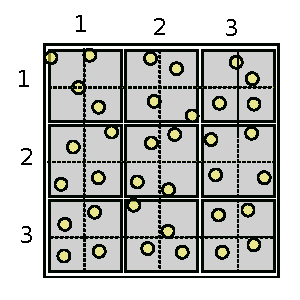
\includegraphics[scale=1]{fig/nonempty_full_quad}
    \caption{Quandrants}
\end{centering} 
\end{figure}

For a sample generated in bin (2,2), in the south-east quadrant, then, assuminb all quadrants of all bins are occupied, the nearest node may be in 

\begin{enumerate}
    \item Any quadrant of bin (2,2)
    \item The northeast quadrant of bin (3,3)
    \item Either of the western quadrants of bin (2,3)
    \item Either of the northern quadrants of bin (3,2)
\end{enumerate}

This is a simple way to narrow down the search, but I'm not sure it will really offer us a gain in runtime. If it does, we can either store four separate kd-trees per bin, or we can add an additional index to the kd-tree which stores the root element of the smallest (hyper-) rectangle (subtree) that fully contains the quadrant.

Nevermind, this is dumb. Rename ``quadrant'' as ``bin'', and all we're advocating here is quadroupling the number of bins.

\section{KD-Tree Implementation}

\begin{figure}[H]
\begin{centering}
    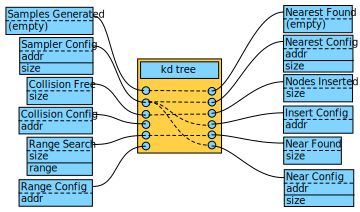
\includegraphics[scale=1]{fig/blocks/kdtree}
    \caption{Sampler Block}
\end{centering}
\end{figure}


The KD tree responds to three signals, and emits three of it's own (not including configuration signals).

\subsection{Samples Generated}
 When the \texttt{Samples Generated} slot is called, it is passed the start address and number of scalar samples that were generated. The kd tree initiates the nearest node search. It will output as many nodes as there are samples generated. It writes the output into an array of result structures. The result structure has the following fields. 

\begin{table}
    \begin{tabular}{|l|l|}
        \hline
        \texttt{state} & n-dim array of the sampled state \\ \hline
        \texttt{node}  & address of the node that was nearest \\ \hline
        \texttt{state} & n-dim array of the nearest node state \\ \hline
        \texttt{collision-free} & boolean \\ \hline
    \end{tabular}
\end{table}

\subsection{Collision Free}
When the \texttt{Collision Free} slot is called, it is assumed that the collision checker has checked all pairs of states in the \texttt{Samples Generated} output array, and has set the \texttt{collision-free} flag in all the pairs for which there is a collision free path between them. The kd tree block then creates a new node in the kd tree for each of the states whose \texttt{collision-free} bit is set to \texttt{true}.

\section{Steering}

For simple steering functions (i.e. for a single integrator) or for functions which cannot be parallelized, in calculating the path from one node to another, the thread who created the sample will be the one who calculates the trajectory. For functions which may be parallelized (i.e. trajectory optimization) we may actually want to serialize over samples, and parallelize the steering of an individual node pair. 

For the single integrator in 2D this is trivial, as the steering is implicit (unless we want to do a distance saturation).

\section{Collision Checking (Single Paths)}

Collision checking may likewise be done in series or parallel. Series has the benefit of aborting early. Is there a bandwidth benefit to parallel collision checking if serial collision checking can maximize throughput?

In the IROS paper we used a kind of brute force collision checking, looking for collisions between all links in all states against all obstacles. This is fine, in general, as it is ``constant'' time (though a large constant). Parallelizing the brute force search is effective, as shown, but we can also potentially use a search index. 


\subsection{Indexed Collision Checking}

Here is an idea for a search index for the 2D Single integrator problem. The idea is to pre-generate a Delauny triangulation of the workspace using the vertices of the obstacles. The edges of the obstacles will naturally be a part of that triangulation and each triangle will be completely in collision or completely free of collision. See figure \ref{fig:delauny}, where the orange edges compose the voronoi decomposition using the vertices of the obstacles and of the workspace. The blue edges connect all vertex pairs which yield a finite-length edge in the vornoi decomposition.  

\begin{figure}[H]
\begin{centering}
    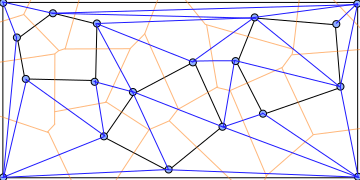
\includegraphics[scale=1]{fig/delauny_collision}
    \caption{Delauny Triangulation}
    \label{fig:delauny}
\end{centering} 
\end{figure}

The blue edges, along with the obstacle edges (black) compose the Delauny triangulation. These is the triangulation which maximizes the minimum angle in all triangles. 

In addition, store the vertices of the obstacles in a search tree (kd-tree) and store a mapping of all vertices to a list of all triangles for which that vertex is a member. 

When we perform a collision check on a query segment, we first find the nearest vertex to one endpoing of the segment. We then find which triangle that has this nearest vertex as one of its members also contains that endpoint. If that triangle is a collision triangle then we exit. If it is not, then we evaluate which of the triangles three edges intersects the segment. We step over that edge and check to see if the next triangle is a collision triangle. We end when we reach the triangle which contains the other endpoint. 

This will only provide a faster search in particular geometric configurations, but I suspect that such configurations are quite common. I suspect it will relate to the ratio of characteristic lengths of obstacles edges, to characteristic lengths of the entire obstacle. 
 

\section{Near Nodes}
\label{a:NearNodes}
Finding near nodes is essentially the same as finding the nearest node, excepting that we're doing a range search on the kd tree. 

However, we need to address the storage of this list. We do not have any kind of built-in centralized allocator that can allocate global memory as needed by each thread. The near node search will generate, in expectation $O(\log n)$ results, which is a growing number. If we allow each sample to store a finite number of near node results, it can lead to very inefficient memory management, and a high probability of a particular near node search running out of memory to store it's results. 

\subsection{Allocator}
We can start by batching up a linked list of near nodes as in  \ref{a:ChildNodeLists} below. If possible, we'd like to find a way to dynamically allocate blocks of near nodes dynamically as threads need them. We can start an array of single blocks, one per thread. Then, once a thread fills up it's local list, we need a way to write that list to a block in global memory, save the per-thread state of the search kernel, and then run a separate kernel to allocate new blocks for all threads that need it. 

Generating a list of all threads that need a new block sounds like a reduction. If, at the end of each call to the search kernel, each thread writes to a boolean whether or not it has filled it's local array, then this is a boolean reduction. It will take $O(\log T)$ to reduce the list of nodes which need a new block allocated, and then a contant amount of time to write to each thread the location of their newly allocated block. 

\begin{figure}[H]
\begin{centering}
    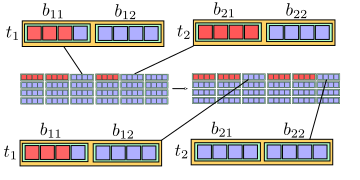
\includegraphics[scale=1]{fig/near_list_allocator}
    \caption{Near List Allocator}
    \label{fig:near_alloc}
\end{centering} 
\end{figure}

Perhaps we can even determine how many iterations to let the search kernel run before checking if the allocation kernel needs to be called. We can do this by running a loop for the number of iterations that we have elements in the thread-level blocks. Then we can perform a thread vote to find out the minimum number of available elements in all threads. If it's zero, then we call the allocator. The allocator allocates a new block to all threads who have at least a full half-block. Then we run the search kernel for another half-blocks worth.

If the block vote results in greater than zero, then we simply recall the search kernel that number of more iterations.
 



\section{Child node lists}
\label{a:ChildNodeLists}
How should we store the child node lists? Does the scheduling of the algorithm yield a reasonable (soft) maximum number of child nodes? If it does, can we enforce such a maximum and still guarentee optimality? What do we do if a desired parent is already saturated, do we find another parent, or do we just drop the node?

Will we hit a huge performance penalty if the child node lists are stored as linked lists? Can we marginalize this penalty by creating a linked list where some $n$ successive entries in that list are stored successively in memory?

\begin{figure}[H]
\begin{centering}
    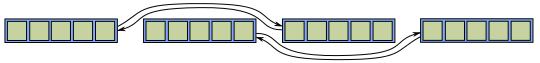
\includegraphics[scale=1]{fig/child_list}
    \caption{Linked-list of arrays}
\end{centering} 
\end{figure}


\section{Rewiring}

Reparenting may lead to a race condition in two ways. 

\subsubsection{On the child}
If a particular node is being considered for rewiring, it is possible that two separate threads have generated ``better'' parents for it. We need to serialize the actual reparenting over the different potentials. 

If all potential rewirings in a particular bin are considered by the thread owning that bin, then this is naturally serialized. However, this will require an exchange of data, since the thread who recognizes that the node should be considered (i.e. the thread that does the near node search) may be a different thread. In addition, the resulting workload will be unbalanced, since some bins will have several potential rewirings while others will have none.


\subsubsection{On the parent}
If a particular newly-sampled node provides a better path for multiple children, then we need to serialize the storage of the child pointers, as the next available pointer may be written by multiple parents. 

If all potential children are enumerated by the thread who sampled the node, this is naturally serialized. I suspect this is the best option. 

\subsubsection{Resolution}
If we store the results of the near-node search as a huge collection of linked lists, as in \ref{a:NearNodes}, then we can the collision checking as a reduction, the same as for the collision check in the sampling phase. For pairs that make it past the collision checking reduction, we may need to sort the pairs to serialize writes to both the child list or for potential reparenting. 

We can make an accessory output of the near node search kernel, or the collision checking kernel, to be the number of nodes returned (the number of potential children, for each retained sample). 

Since the race condition on parenting will actually result in throwing out evaluated connections, we can treat this as a reduction as well. It essentially ammounts to finding all rewirings that end at node $i$, and then picking the one that is best. This can be done by sorting the end points of all the remaining near node searches (a reduction sort), and then reducing all repetitions (a min reduction). 
 
\begin{figure}[H]
\begin{centering}
    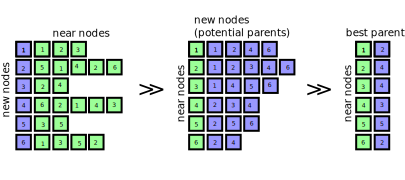
\includegraphics[scale=1]{fig/kernel_near_rotate}
    \caption{Near Reduction}
\end{centering} 
\end{figure}

Merge sort should be easy to parallelize. After the nodes are sorted then we can run a second kernel to generate start points and lengths for each array. Each thread can look at a pair of elements and see if they have different parents. If they do, it marks an end/start of an array. Then we can run a reduction on the output of that kernel to get a simple array of start addresses and end adddresses. 

After this, all potential race conditions on reparenting the potential child will be resolved. Then we can perform another reduction sort to put the search results back in parent ordering. Then we can assign one thread per parent to write the children to the child list, using the same synchronized allocator as before. 
 
\begin{figure}[H]
\begin{centering}
    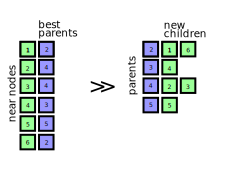
\includegraphics[scale=1]{fig/kernel_parent_rotate}
    \caption{Parent Reduction}
\end{centering} 
\end{figure} 


\section{Cost propogation}
If the result of all reparenting operations is performed as above, the result of the child race-resolution kernel can be reused as the initial data set for the cost propogation kernel. Again, we can use the linked list marginalization strategy to batch up nodes that need updating. Each kernel that touches a node adds to it's list of children that now need to be updated. If that list gets too big, it writes the excess to global memory, and asks the allocator for a new block to write it's next excess. If it ever expires its list, it asks the allocator for a new read-block.





\end{document}

 